\section{Opis stworzonego systemu}\label{rozdzial_system}
W~niniejszym rozdziale opisana jest realizacja systemu stworzonego przez autora pracy. W kolejnych podrozdziałach znajdują się opisy poszczególnych jego elementów oraz użytych narzędzi.

\subsection{Schemat systemu}
Na rysunku \ref{systemSchemeImage} przedstawiony został schemat stworzonego systemu, który posłużył do realizacji klasyfikacji utworów muzycznych. Pokazuje on ogólny zamysł zaproponowany przez autora w~celu rozwiązania problemu rozpoznawania nastroju muzyki. Pierwszym krokiem, który należy podjąć jest wstępna obróbka utworów muzycznych, a~następnie wyekstrahowanie ich cech dźwięków. Na podstawie takie bazy danych należy podzielić dane na zbiór uczący oraz testowy, które będą służyć kolejno do uczenia sieci neuronowej, a~następnie do jej oceny przez klasyfikator, którym jest sieć neuronowa.

\begin{figure}[ht!]
\centering
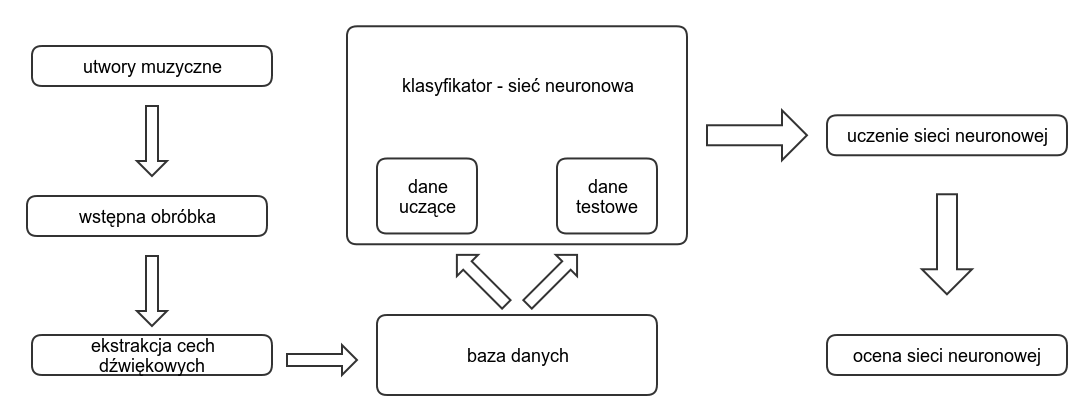
\includegraphics[scale=0.4]{res/systemScheme.png}
\caption{Schemat systemu}\label{systemSchemeImage}
\end{figure}

\subsection{Zastosowane narzędzia}
W~celu zbudowania systemu rozpoznającego nastrój muzyki należało wybrać język programowania oraz biblioteki umożliwiające analizę utworów muzycznych, ekstrakcję potrzebnych cech, a~także implementujące sztuczne sieci neuronowe. Ponadto, niezbędny był wystarczająco duży zbiór utworów muzycznych, który mógłby posłużyć jako baza danych systemu.

\subsubsection{Język programowania oraz biblioteki programistyczne}
Język programowania jest językiem w~którym człowiek może komunikować się z~komputerem i~przez to ,,kazać'' mu wykonać  określone zadanie. Niewątpliwie dobrze jest posiadać swobodę w~porozumiewaniu się tym językiem i~ten argument spowodował, że wybór padł na język programowania Python, który jest językiem wysokopoziomowym ogólnego przeznaczenia, który zdobywa coraz większą popularność. Jest to spowodowane jego prostą oraz dużymi możliwościami, co w połączeniu z~dostępnymi bibliotekami naukowymi (matplotlib, numpy) powoduje, że staje się on dużą konkurencją dla popularnego Matlaba. W parze z~językiem programowania idą także biblioteki programistyczne. W~niniejszej pracy największą rolę odegrały dwie z nich tj. biblioteka Essentia\cite{essentia} oraz NeuroLab. Pierwsza z~nich została napisana w~języku C++, ale oferuje także tzw. bindingi, które pozwalala na jej użycie także w~języku Python. Posiada ona szeroką gamę algorytmów wykorzystywanych w~analizie dźwięków i~w~tym celu została użyta w~tej pracy,a~także wielu innych związanych z MIR\footnote{MIR - Music Information Retrieval}. Druga natomiast, jest prostą i~potężną biblioteką implementującą sieci neuronowe. Obie znacznie ułatwiły pracę nad problemem podjętym w~niniejszej pracy.

\subsubsection{System operacyjny}
Systemem operacyjnym użytym przy realizacji założonego zadania był system Linux, dokładnie dystrybucja Xubuntu. Przenośność języka programowania jakim jest Python pozwala jednak na używanie aplikacji także na ich systemach pod warunkiem zainstalowania koniecznych do jego działania bibliotek jakimi są wspomniane biblioteki: Essentia oraz NeuroLab.

\subsubsection{Baza utworów muzycznych}
Koniecznością było pozyskanie odpowiedniej bazy danych, aby móc z jej wykorzystaniem nauczyć oraz przetestować sieć neuronową. Pierwszym pomysłem był odsłuch i~ocena utworów przez samego autora i~ewentualną osobę towarzyszącą. Biorąc jednak pod uwagę wysoką subiektywność percepcji muzyki prawdopodobnie nie byłby to miarodajny osąd. Z~pomocą przyszedł zbiór danych\cite{dataSet} zawierający 744 utwory różnych gatunków muzycznych opublikowany właśnie dla prac naukowych o~tematyce zbliżonej do niniejszej pracy. Wszystkie fragmenty zbioru pozyskane zostały z~otwartego archiwum muzyki\footnote{Free Music Archive - \url{http://freemusicarchive.org/}}. Każdy z~utworów jest 45-cio sekundowym fragmentem uzyskanym z~pełnego utworu oraz ocenionym zarówno pod względem pobudzenia jak i~zadowolenia przez ponad 300 osób. Skala ocen należy do przedziału $[1,9]$ dla obu parametrów, a~każdy uczestnik przeprowadzonego badania oceniał utwór w czasie ciągłym\footnote{\url{https://www.youtube.com/watch?v=G-GhONd_Wag}}, co dawało średnią częstotliwość oceniania 2~Hz biorąc pod uwagę możliwości techniczne przeglądarek internetowych oraz komputerów używanych przez badanych. Wszystko to sprawia, że ten zbiór danych stanowił dobrą podstawę dla systemu tworzonego przez autora. 

\subsubsection{Algorytm uczenia maszynowego}
Temat pracy brzmi ,,Wykorzystanie uczenia maszynowego do rozpoznawania nastroju muzyki''. Algorytmem, który jednak został wybrany do realizacji tego celu, zostały sztuczne sieci neuronowe, które pozwalają na pozostawienie problemu implementacji rozwiązania problemu samej sieci, co jest znacznym ułatwieniem.

\subsection{Opis aplikacji}
Pierwszy etapem działania programu jest wczytanie utworów muzycznych, które są zapisane w formacie mp3. Po tym następuje ich wstępna obróbka, która obejmuje zastosowanie okna czasowego dla przetwarzanego sygnału oraz algorytm wyrównywania poziomu głośności. Po wstępnej obróbce, obliczony zostaje wskaźnik zmiany znaku oraz wskaźnik zmian po której wykonywana jest transformacja Fouriera w celu otrzymania widma sygnału, które jest niezbędne w~celu obliczenia kolejnych cech dźwiękowych, którymi są kolejno złożoność spektralna, dysonans, skala, płaskość spektralna oraz kształt spektralny w którego skład wchodzą środek masy widma, współczynnik skośności widma, kurtoza widma, \emph{roll off} widma oraz rozrzut widma. Po ekstrakcji cech następuje uczenie oraz testowanie sieci neuronowej. W~tym celu baza utworów została podzielona na dwa zestawy, pierwszy z nich składa się 674 utworów służących do uczenia sieci neuronowej, natomiast drugi z 70 utworów, który służy jako zestaw do oceny sieci neuronowej. Na wejście sieci, zbudowanej z wykorzystaniem biblioteki NeuroLab, przekazywane są wyżej wymienione cechy. Jednokierunkowa sieć neuronowa (ang. \emph{feed-forward}) zwraca dwie wielkości: zadowolenie oraz pobudzenie, które opisują nastrój reprezentowany przez utwór. Wszystkie oceny badanych z wykorzystywanej bazy danych zostały przeskalowane do przedziału $[-1,1]$, ponieważ została użyta tangensoidalna funkcja aktywacji. Użycie liniowej funkcji aktywacji znacznie ogranicza możliwości sieci, co jest spowodowane tym, że funkcja modelowana przez złożenie funkcji liniowych wciąż pozostanie liniowa, natomiast funkcję liniową można modelować pojedynczym liniowym neuronem z czego wynika wniosek, że wielowarstwowa topologia zwiększa możliwości tylko w przypadku użycia nieliniowych funkcji aktywacji.

\subsection{Uczenie sieci neuronowej}
Jednym z~podstawowych zadań przy treningu sieci neuronowej jest dobór optymalnej topologii sieci, a~w~szczególności liczby neuronów w~warstwie ukrytej. Istnieją ogólne reguły jak należy w~tym wypadku postępować. 
Z~całą pewnością liczba neuronów w~warstwie ukrytej nie powinna być zbyt duża ani zbyt mała. Zbyt duża, to znaczy znacznie przekraczająca ilość neuronów wejściowych, ponieważ może to spowodować przeuczenie sieci neuronowej. Przeuczenie, lub też przetrenowanie, sieci polega na tym, że będzie ona nadmiernie dopasowana do danych uczących przez co nie będzie odporna na szumy. Można powiedzieć, że sieć nauczy się ,,na pamięć'' wyników dla danego zestawu danych, co nie jest oczekiwanym rezultatem. Zbyt mała liczba neuronów oznacza liczbę neuronów znacznie mniejszą od ilość neuronów wejściowych. Nie pozwoli to sieci odpowiednio modelować poszukiwanej zależności pomiędzy jej wejściami , a~wyjściami. W~przypadku uczenia znaczenie ma także czynnik losowy, ponieważ wagi sieci inicjalizowane są wartościami losowymi. Biorąc pod uwagę wspomniane fakty, w celu nauczenia sieci neuronowej wykonany został skrypt korzystając z języka skryptowego powłoki systemowej UNIX, który pozwalał na automatyczne wielokrotne uruchamianie programu. Korzystając z dostępnych flag sprawdzane były także wyniki uzyskiwane przez sieć dla różnej liczby neuronów w warstwie ukrytej. Użytym kryterium oceny sieci była wartość funkcji minimalizowanej przez algorytm uczący, która jest przedstawiona we wzorze \ref{minFunc}.

Na wykresie \ref{error} przedstawiona została wartość minimalizowanej funkcji w~zależności od liczby iteracji. Łatwo można zauważyć, że już od około setnej iteracji sieć neuronowa praktycznie przestaje się uczyć, następują już wtedy tylko nieznaczne zmiany. Ostatecznie, najmniejsza uzyskana wartość błędu wynosi $4.299$ dla zbioru testowego oraz $31.303$ dla zbioru uczącego. Najlepszy wynik został otrzymany dla sieci o~liczbie neuronów w~warstwie ukrytej równej 7. Łatwo jest jest też doprowadzić do sytuacji przeuczenia sieci. W przypadku uruchomienia programu z~40~neuronami w~warstwie ukrytej otrzymujemy błędy $13.426$; $10.575$ kolejno dla zestawu uczącego oraz testowego. Jak łatwo zauważyć, pomimo tego, że mogłoby się wydawać, że sieć dużo lepiej została wytrenowana, to jedna wyniki dla zestawu testowego są gorsze niż w~przypadku tej pozornie gorzej wytrenowanej. W tabeli \ref{table:przeuczenie} przedstawione zostały wartości błędu dla zestawów uczących oraz testowych dla sieci z 40 neuronami oraz z~7~neuronami podzielone przez liczbę utworów uczących oraz testowych. Widać tutaj sporą różnicę pomiędzy błędem dla zestawu testowego oraz uczącego w~przypadku sieci z 40 neuronami, co wskazuje zdecydowanie na jej przeuczenie.

\begin{table}
\centering
\begin{tabular}{|c|c|c|}
\hline
 liczba neuronów sieci & 40 & 7 \\ 
 \hline
% błąd dla 70 utworów uczących & $1.38$ & $3.445$ \\  
błąd dla utworów uczących / liczba utworów uczących & $0,012$ & $0.050$ \\  
 \hline
% błąd dla 70 utworów testowych & $10.575$ & $4.299$ \\ 
błąd dla utworów testowych / liczba utworów testowych & $0.15$ & $0.061$ \\ 
 \hline  
 \end{tabular}
 \caption{Błąd dla 70 utworów dwóch różnych sieci} \label{table:przeuczenie}
\end{table}


\begin{figure}[ht!]
\centering
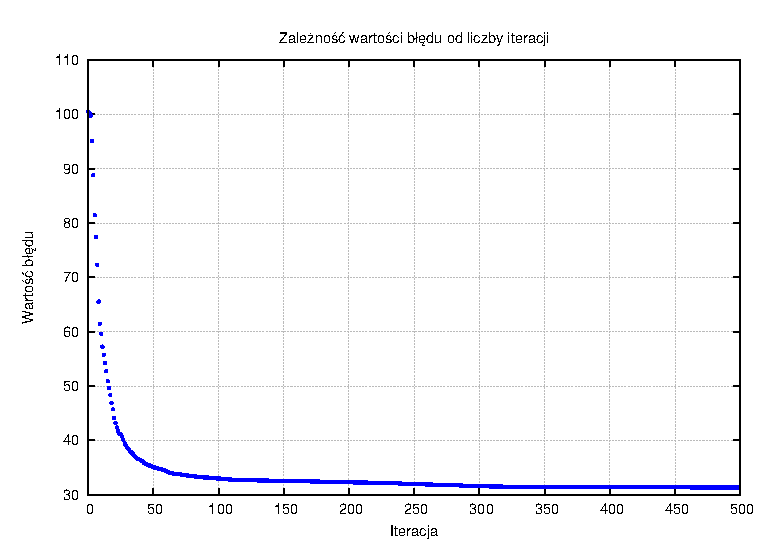
\includegraphics[scale=1.27]{res/error.eps}
\caption{Zależność wartości błędu od liczby iteracji\label{error}}
\end{figure}

